\documentclass{article}
\usepackage[utf8]{inputenc}
\usepackage{amsfonts}
\usepackage{amsmath}
\usepackage{amssymb}
\usepackage[T1]{fontenc}
\usepackage{tgpagella}
\usepackage{graphicx}
\usepackage{fullpage}
\usepackage{mathtools}
\usepackage{ dsfont }
\usepackage{verbatim}

\title{Proof of Quicksort Correctness}
\author{Brendan Ritter}
\date{December 2013}

\begin{document}

\maketitle
\section{Introduction}
Human beings like order. We like being able to type something into google and get out what we expect. The majority of our ability to find things in the systems we have made is due to sorting algorithms. One of the most commonly used sorting algorithms is quicksort.
\\\\
Quicksort is named so because it is generally faster than most other sorting algorithms in most cases. For this paper we will consider the quicksort algorithm and prove how it is a valid sorting algorithm, as well as defining the algorithm in a somewhat rigorous manner. Note that there is also a in-place version of Quicksort and various ways of choosing the pivot. The definition presented below is not in place and chooses the first element to be the pivot for simplicity.


\section{Less Rigorous Definition of Quicksort}
This is a definition that can be done with pen and paper. Try it out and see for yourself. An example of steps is incuded in the Implementation section further down.
\\\\
You have a list of numbers. If that list of numbers has one element it is already sorted. If not, take the first element in your list. Compare that first element to the others in the list.
\\\\
Make one list of elements less than the first and another list of elements greater than the first. Sort those two lists in the same manner. Concatenate the sorted less list and the first element and the sorted greater list. Your entire list is now sorted. 


\section{More Rigorous Definition of Quicksort}
In order to prove the correctness of quicksort, we need a definition of quicksort to work with. I have defined a simple version based off the description in wikipedia with the implementation of choosing my pivot to be the first element to make things easier.
\\\\
Let $Input$ be a tuple of length $n$ where for all element $a$ of $Input$, $a \in \mathds{R}$, in other words, $Input=(a_{1}...a_{n})$
\\\\
Define a function $Quicksort$ such that:
\\
\[
 Quicksort(Input) =
  \begin{cases}
   Input                      & \text{if } n \leq 1 \\
   Partition(Input)       & \text{otherwise}
  \end{cases}
\]
Define a further function $Partition$ that accepts a tuple and preforms the following operations:
\begin{itemize}
\item Remove the first element of $Input$. This is $a_{1}$ and will be the pivot.
\item Define two new tuples in the following manner: for all element $a$ except $a_{1}$ in $Input$, if $a \leq a_{1}$ then $a \in less$ and if $a \textgreater a_{1}$ then $a \in more$.
\\\\
In other words, $less$ contains all elements of $Input$ which are less than or equal to the first element of $Input$ and $more$ contains all elements of $Input$ which are greater than the first element of $Input$. 
%\item Define a new tuple $less=(b_{0}...b_{n})$ such that for all $b$ in $less$, $b \in Input$ and $b \leq a_{1}$. In other words, $less$ contains all elements of $Input$ which are less than or equal to the first element of $Input$.  
%\item Define a new tuple $more=(c_{0}...c_{n})$ such that for all $c$ in $more$, $c \in Input$ and $c \textgreater a_{1}$. In other words, $more$ contains all elements of $Input$ which are greater than the first element of $Input$. 

\item Let $sortedLess= Quicksort(less)$
\item Let $sortedMore=Quicksort(more)$
\item $Partition(Input)$ returns $sortedLess+(a_{1})+sortedMore$. 
\end{itemize}
$(a_{1})$ is the singleton tuple containing only the first element of $Input$, our pivot. In addition, the $+$ is being used to denote concatenation. For example $(1,2,3)+(9,3)=(1,2,3,9,3)$


\section{What We Want to Prove}
So we have our definition of quicksort. Now we want to prove three things. Firstly, we want to know that regardless of input, quicksort will finish its calculation. It wouldn't be very useful if you input a tuple to be sorted and the function never ended.
\\\\
Since quick sort is in fact a sorting algorithm, it must meet the requirements for a sorting algorithm. Quicksort's output needs to be a permutation of its input (no elements dropped or inserted). Finally, the output needs to be sorted; the output needs to be in non-decreasing order (no element is smaller than the previous)
\\\\
These three fact will be proven using induction on the number of elements of the input. Theoretically they could be lumped into one giant induction. However, for clarity's sake I have separated them.

\section{Termination}
In order to prove the correctness of quicksort we need to make sure that in the definition defined above, there are no infinite loops (since quicksort calls itself, how do we know that its evaluation ever ends?)
\\\\
We will continue using induction on the number of elements in $Input$, that value was defined above as $n$.
\\\\
\textbf{Base Case:} \\
The length of $Input$ is less than or equal to 1. In other words $n\leq 1$. \\
If this is the case, then we know that $Quicksort$ will halt because it simply returns $Input$.
\\\\
\textbf{Inductive Hypothesis:}\\
$Quicksort(Input)$ will halt for all $Input$ of size $n<=k$.
\\\\
\textbf{Inductive Step:}\\
Consider an input tuple of size $n=k+1$. 
Since n is larger than 1, it would run $Partition()$.
Regardless of the value of $a_{1}$ however, I assert that both $less$ and $more$ need to be at most of size $\textless n$. This is because the input tuple was of size n.Then the pivot of $a_{1}$ is chosen. Since $less$ is defined to be all the elements of $Input$ that are less than $a_{1}$, even if all elements are less than $a_{1}$, since we 'took out' $a_{1}$. at most $less$ can be of size $n-1$.
\\\\
Similarly, even if all elements are more than $a_{1}$, since we took out $a_{1}$, at most $more$ can be of size $n-1$.
\\\\
Since we have shown that given any values for $a_{1}$ through $a_{n}$, the recursive calls will always be made on tuples of at most, size $n-1$ and since we know for this case that $n=k+1$, that means that at most recursive calls will be made on tuples of size $n=k$. From our inductive hypothesis we know that $Quicksort$ of any $n<=k$ halts, therefore, the recursive calls will always halt also. 
\\\\
All that is required then, is the concatenation of the two recursive calls. Thus, $Quicksort(Input)$ for any arbitrary size $Input$ will halt. 

\section{Permutation}
In order to be a sort $Quicksort(Input)$ must be some permutation of $Input$. This means that no elements can be dropped or added. Every element in the input is present in the output.
\\\\
We can continue again with induction on the number of elements in $Input$.\\\\
\textbf{Base Case:} \\
The length of $Input$ is less than or equal to 1. On way this is possible is if the input is the empty tuple (), and quicksort returns (). () is a permutation of (). The other possibility is that $Input$ was a singleton tuple. In that case $quicksort$ returns that same singleton list. This is also a valid permutation since nothing has changed.
\\\\
\textbf{Inductive Hypothesis:}\\
The output of $Quicksort$ for any input tuple of size $n<=k$ is a permutation of the input.
\\\\
\textbf{Inductive Step:}\\
Consider an input tuple of size $n=k+1$.\\
Since $n$ is larger than 1, it would run $Partition()$.
We must then keep track of the elements of $Input$. The first thing that happens in $Permutation$ is that we remove the first element of $Input$, however, looking ahead at the return statement, we see that this value is specifically added back in.
\\\\
The rest of the elements are then divided up between $less$ and $more$. I claim that by definition of  $less$ and $more$ that all elements in $Input$ except for $a_{1}$ are either in $less$ or $more$. Thus, no element is dropped when going to $less$ and $more$ except for $a_{1}$. 
\\\\
Next, $less$ and $more$ are sorted. Since we know the sorted versions of $less$ and $more$ will be at largest, one element smaller than $Input$ (of size $n=k$), our inductive hypothesis says that $sortedLess$ and $sortedMore$ are permutations of $less$ and $more$. This means that no elements are dropped or added in the recursive sorting process. 
\\\\
Finally, we concatenate $sortedLess$, $a_{1}$ and $sortedMore$. Since every element in $Input$ was either in $less$, $more$ or was $a_{1}$, the concatenation of all three of those tuples will hold all elements in $Input$, and no more, since none were added. Thus, we can conclude that for a tuple of size $n=k+1$, and by induction, all tuples of finite but arbitrary length, the output of $Quicksort$ will be a permutation of $Input$.

\section{Ordination}
To be a sort, $Quicksort$'s output must be in nondecreasing order. I will use the word 'order' to describe nondecreasing order. \\
Like before, we will continue with induction.\\\\
\textbf{Base Case:}\\
The length of $Input$ is less than or equal to 1. If $Input$ is (), then it is already ordered and $Quicksort$ outputs (). If $Input$ is a singleton tuple $(a)$, then it is also already in nondecreasing order. 
\\\\
\textbf{Inductive Hypothesis:}\\
Given $Input$ is of length $n \textless k$, $Quicksort(Input)$ is in nondecreasing order.
\\\\
\textbf{Inductive Step:}\\
Consider a tuple of length $n=k+1$. We want to show that $Quicksort$ of this tuple gives an output in nondecreasing order. \\\\
Since $n$ is larger than 1, it would run $Partition()$.
We now need to analyze the order in which the elements are placed. When we construct $less$ and $more$, notice that by definition, all elements in $less$ are in fact less than or equal to our pivot $a_{1}$ and all the elements in $more$ are greater than $a_{1}$.
\\\\
Now that we know that $less$, $a_{1}$ and $more$ are in the right order in relation to one another, we need to ensure that by taking $Quicksort$ on $less$ and $more$ we don't disturb that order. For this, we use our prior proof that the output of $Quicksort$ is merely a permutation of the input, for any size input. Because of this, we know that there exists no element in $sortedLess$ that is larger than $a_{1}$ and no element in $sortedMore$ that is less than $a_{1}$.
\\\\
Finally we need to prove that internally that all elements of $sortedLess$ and $sortedMore$ are in nondecending order. This is proven by our inductive hypothesis. Since once again, $less$ and $more$ are tuples of size $n=k$, our inductive hypothesis applies and says that $Quicksort$ of those tuples will be in nondecreasing order.
\\\\
I claim that due to the previous two facts, the concatenation of $sortedLess$, $a_{1}$ and $sortedMore$ needs to result in a tuple of nondecreasing elements. Thus, $Quicksort$ of all tuples of size $k+1$ are ordered. Finally, by induction, we can conclude for all input tuples of finite but arbitrary length, the output of $Quicksort$ will be a tuple of nondescending order.
\pagebreak
\section{Implementation}
\textbf{By hand}
\begin{figure}[h!]
\centerline{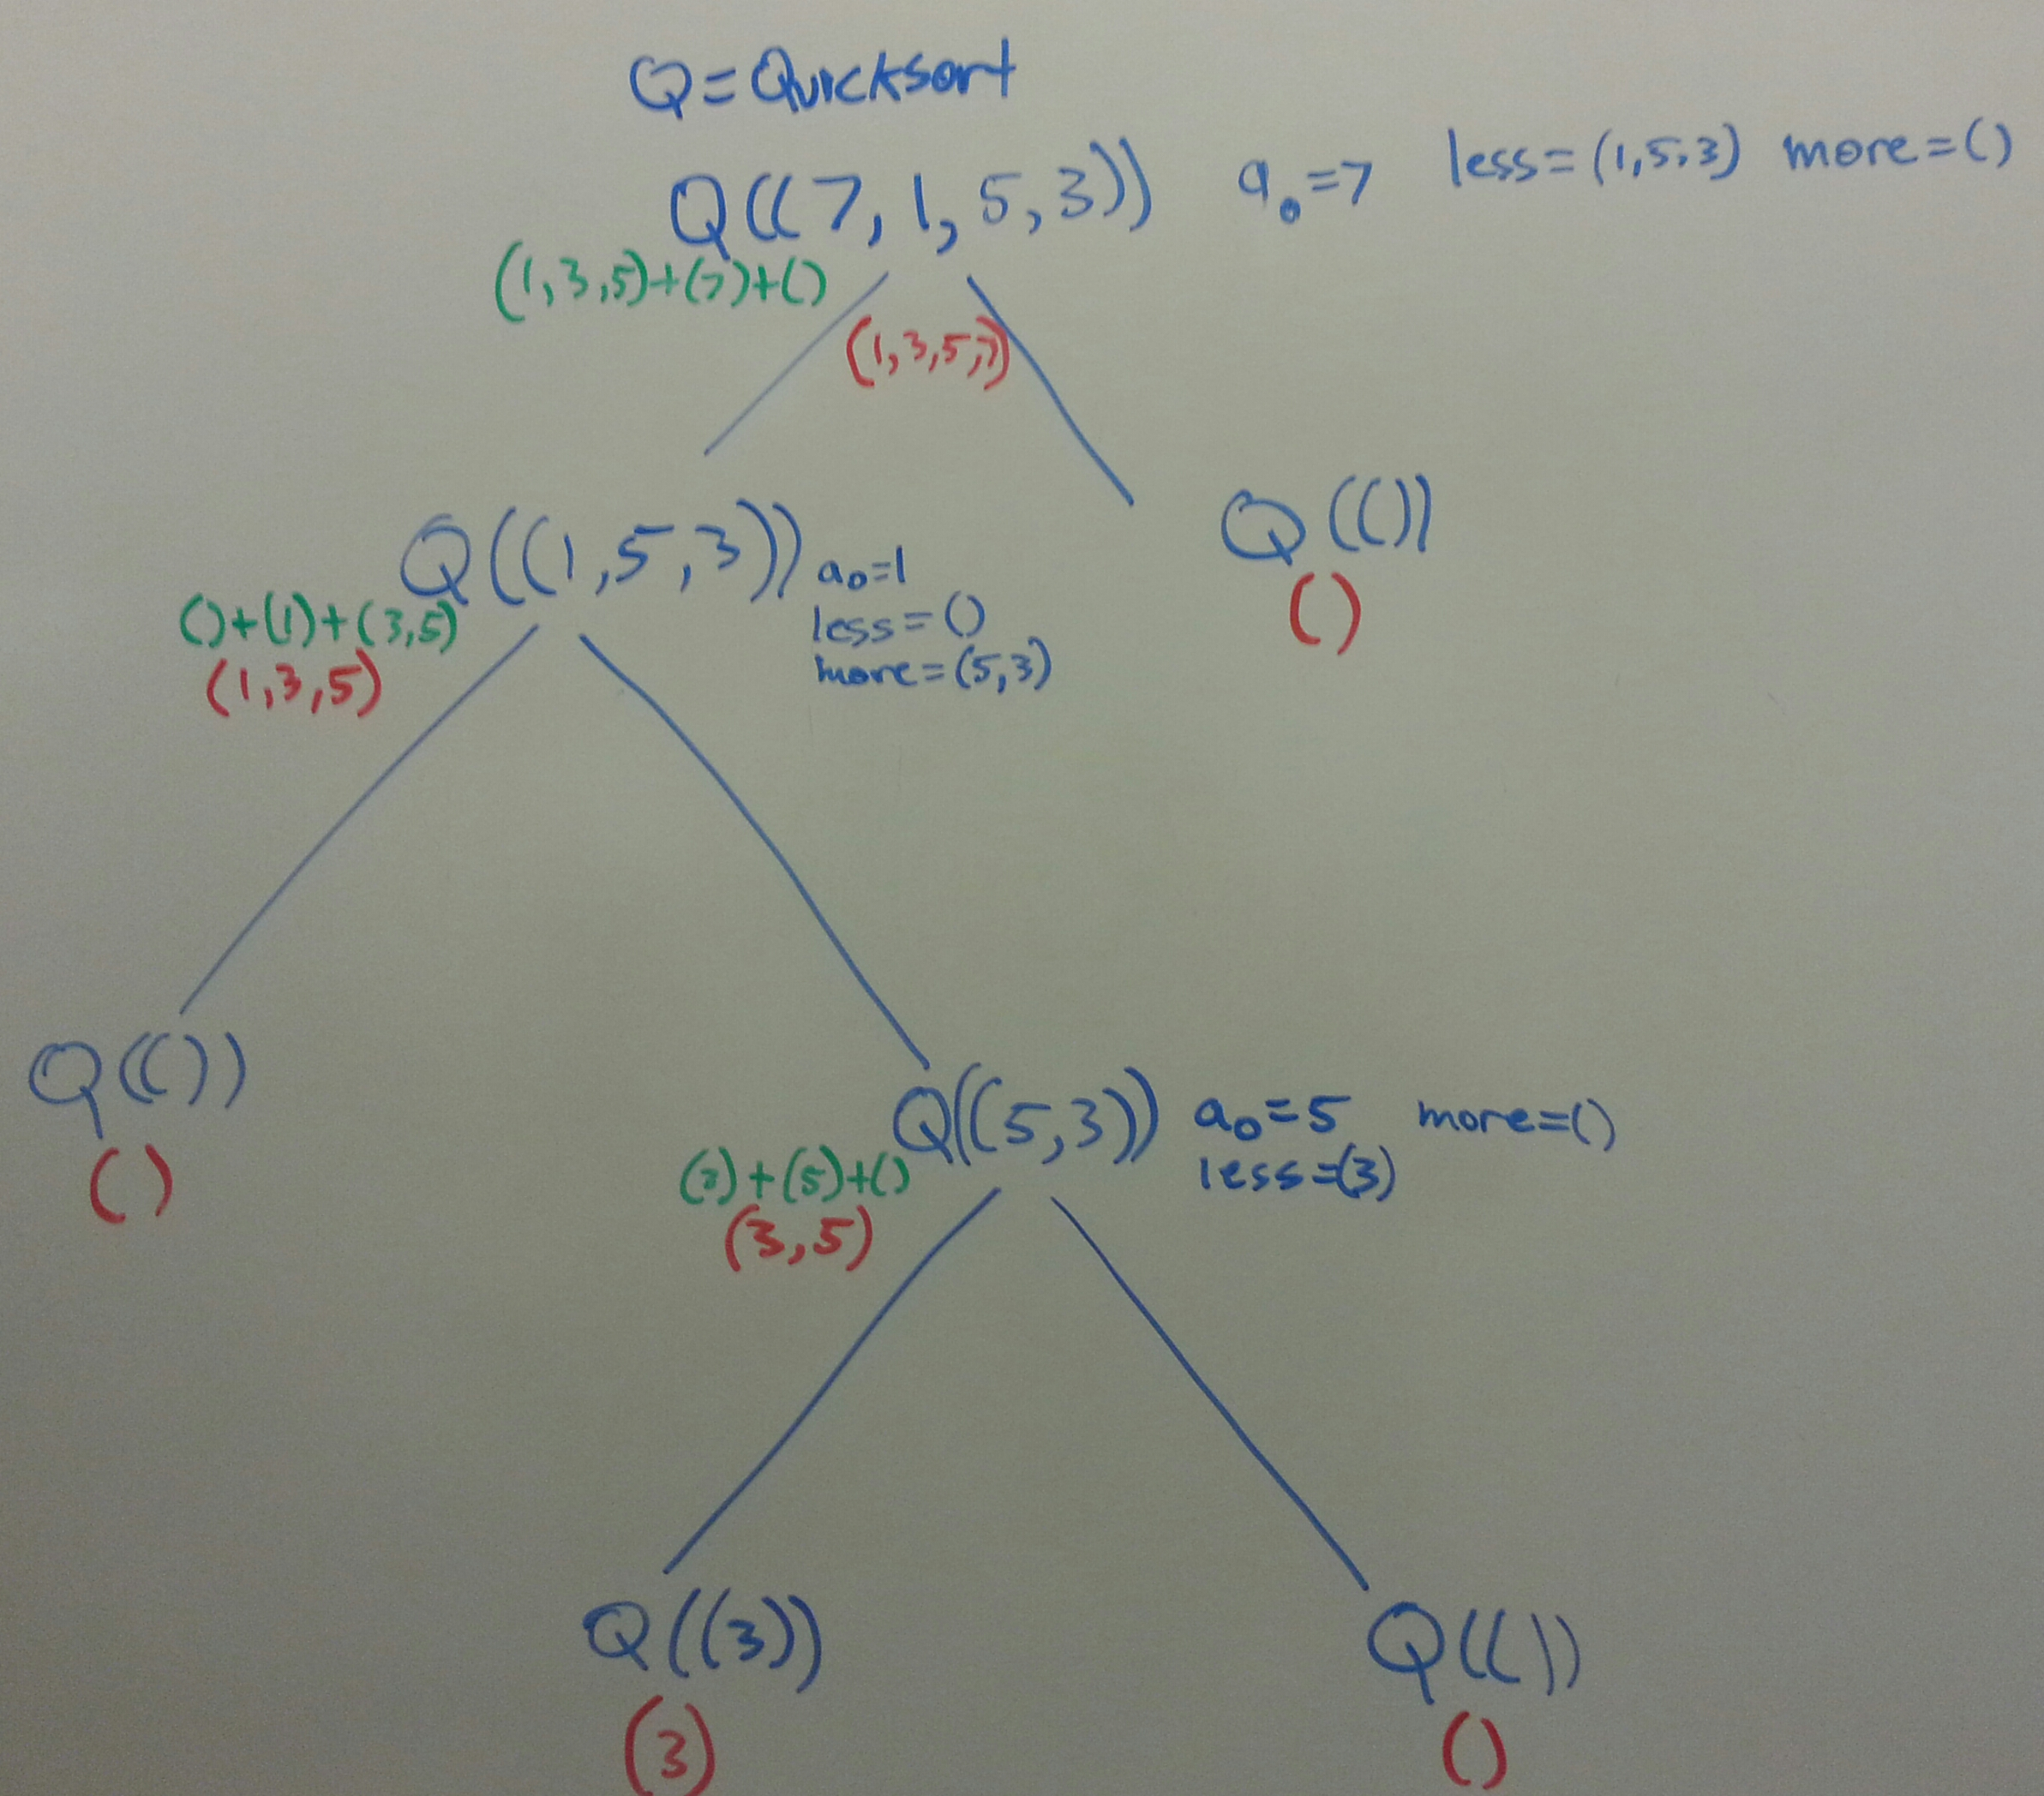
\includegraphics[height = 3.5 in]{Quicksort.jpg}}
\caption{Showing the recursive calls on the tuple (7,1,5,3). The numbers in red are the result of each call, the 'local variables' are shown when $Partition$ is used to calculate the answer.}
\end{figure}
\\\\
\textbf{Python}\\
In order to understand the algorithm better, I have included an implementation of quicksort in Python.
\\
\begin{verbatim}
import math

def quicksort(input_array):
	    if len(input_array)<=1:
		        return input_array
	    pivot=input_array.pop(0)
	    less=[]
	    greater=[]
	    for el in input_array:
		        if el <=pivot:
			            less.append(el)
		        else:
			            greater.append(el)
	    return quicksort(less)+[pivot]+quicksort(greater)

def main():
	    print quicksort([7,3,-2.7777,6,-98,8.5,42,6,math.pi,78,0,
		    "Why_is_there_a_string_here?","This is crazy",[1,2],(3,4,5)])

if __name__ == '__main__':
	    main()
\end{verbatim}
The output of the above script should produce:\\
\begin{verbatim}
[-98, -2.7777, 0, 3, 3.141592653589793, 6, 6, 7, 8.5, 42, 78, [1, 2], 
'This is crazy', 'Why_is_there_a_string_here?', (3, 4, 5)]

\end{verbatim}
Note that the implementation above is very flexible and handles perfectly several possible edge cases:
\begin{itemize}
\item Negative numbers
\item The number $\pi$
\item Negative and positive decimals
\item Equal numbers (6)
\item It even handles crazy inputs like strings, tuples and lists.
\end{itemize}
The last crazy inputs are included to show that it doesn't matter what is being sorted as long as there exists a comparison between them. 
\\\\
In this case the comparing operators in Python (<,<=,>,>=) are overloaded to allow comparison between seemingly incomparable types simply using by the alphabetical order of the class name. Thus (L)ist comes before (S)tring, which comes before (T)uple. Numeric types always always come before non-numeric ones.  
\end{document}



















